\documentclass[11pt,openany]{book}

% ----- Packages -----
\usepackage[a4paper,margin=1in]{geometry}
\usepackage[T1]{fontenc}
\usepackage{amsmath,amssymb,amsthm}
\usepackage{graphicx}
\usepackage{xcolor}
\usepackage{booktabs}
\usepackage{array}
\usepackage{tabularx}
\usepackage{enumitem}
\usepackage{listings}
\usepackage{tcolorbox}
\tcbuselibrary{breakable,skins}
\usepackage{tikz}
\usetikzlibrary{trees,positioning,arrows.meta,shapes.geometric,calc,shadows}
\usepackage{hyperref}
\hypersetup{colorlinks=true,linkcolor=blue!60!black,urlcolor=blue!60!black,
            citecolor=blue!60!black,linktoc=all}
\usepackage{caption}
\usepackage{titlesec}
\usepackage{fancyhdr}
\usepackage{textcomp}

% ----- Listings setup -----
\definecolor{codebg}{RGB}{248,248,248}
\definecolor{codecomment}{RGB}{0,128,0}
\definecolor{codekw}{RGB}{0,0,180}
\definecolor{codestr}{RGB}{163,21,21}

\lstdefinestyle{cudastyle}{
  basicstyle=\ttfamily\small,
  backgroundcolor=\color{codebg},
  commentstyle=\color{codecomment}\itshape,
  keywordstyle=\color{codekw}\bfseries,
  stringstyle=\color{codestr},
  numbers=none,
  showstringspaces=false,
  breaklines=true,
  frame=single,
  rulecolor=\color{black!30},
  framesep=4pt,
  xleftmargin=4pt,
  xrightmargin=4pt,
  language=C++,
  morekeywords={__global__,__device__,__host__,blockIdx,threadIdx,blockDim,gridDim,
                __syncthreads,__threadfence,proc,procedure,for,while,if,else,parallel,
                in,from,to,downto,by,scan,prescan,split,reduce,permute,return}
}
\lstset{style=cudastyle}

% ----- Box environments -----
\newtcolorbox{notebox}{
  enhanced, breakable, colback=blue!4, colframe=blue!50!black,
  boxrule=0.4pt, arc=2mm, left=6pt, right=6pt, top=4pt, bottom=4pt,
  before skip=8pt, after skip=8pt
}
\newtcolorbox{pitfallbox}{
  enhanced, breakable, colback=red!4, colframe=red!60!black,
  boxrule=0.4pt, arc=2mm, left=6pt, right=6pt, top=4pt, bottom=4pt,
  before skip=8pt, after skip=8pt
}
\newtcolorbox{keyideabox}{
  enhanced, breakable, colback=green!4, colframe=green!50!black,
  boxrule=0.4pt, arc=2mm, left=6pt, right=6pt, top=4pt, bottom=4pt,
  before skip=8pt, after skip=8pt
}
\newtcolorbox{examplebox}{
  enhanced, breakable, colback=orange!4, colframe=orange!70!black,
  boxrule=0.4pt, arc=2mm, left=6pt, right=6pt, top=4pt, bottom=4pt,
  before skip=8pt, after skip=8pt
}
\newtcolorbox{exercisebox}{
  enhanced, breakable, colback=purple!4, colframe=purple!50!black,
  boxrule=0.4pt, arc=2mm, left=6pt, right=6pt, top=4pt, bottom=4pt,
  before skip=8pt, after skip=8pt
}

% ----- Header / footer -----
\pagestyle{fancy}
\fancyhf{}
\fancyhead[LE,RO]{\thepage}
\fancyhead[RE]{\nouppercase{\leftmark}}
\fancyhead[LO]{\nouppercase{\rightmark}}
\renewcommand{\headrulewidth}{0.4pt}
\setlength{\headheight}{14pt}

% ----- Title spacing -----
\titlespacing*{\chapter}{0pt}{-20pt}{20pt}

% ----- Document -----
\begin{document}

% ============ TITLE PAGE ============
\begin{titlepage}
  \begin{center}
    \vspace*{2cm}
    {\Huge \bfseries Parallel Programming\par}
    \vspace{0.6cm}
    {\Large Concepts, Patterns, and\\ Practice\par}
    \vfill
    {\large Author Name\par}
    \vspace{0.5cm}
    {\large April 25, 2026\par}
  \end{center}
\end{titlepage}

% ============ COPYRIGHT PAGE ============
\thispagestyle{empty}
\noindent\textbf{Copyright}\\[1em]
Copyright \textcopyright\ 2026 Author Name.\\[0.5em]
All rights reserved.\\[0.5em]
No part of this book may be reproduced, stored in a retrieval system, or
transmitted in any form or by any means, electronic, mechanical, photocopying,
recording, or otherwise, without prior written permission of the publisher,
except for brief quotations in reviews.\\[0.5em]
First edition: 2026
\clearpage

% ============ TABLE OF CONTENTS ============
\frontmatter
\setcounter{tocdepth}{2}
\tableofcontents
\clearpage

% ============ MAIN CONTENT ============
\mainmatter
\setcounter{chapter}{5}

\chapter{Lecture 24: Parallel Algorithms --- Prefix Sum and Radix Sort}

\section{Overview}
This lecture introduces two foundational parallel algorithms that appear
repeatedly throughout the design of modern parallel and distributed
systems: \textbf{parallel prefix sum} (also called \emph{scan}) and
\textbf{parallel radix sort}. Prefix sum is a deceptively simple operation
that, despite appearing inherently sequential, admits efficient parallel
algorithms with $O(\log_2 n)$ depth. We study two classical algorithms ---
the \emph{Hillis \& Steele} algorithm (1986) and the \emph{Blelloch} algorithm
(1990) --- and analyse their work, depth, and PRAM complexity. Radix sort, a
non-comparison-based sorting algorithm, is then shown to be a natural client
of parallel scan: its key step (the \emph{scatter}) depends on a prefix-sum
over a histogram of digit counts.

\section{Key Learning Outcomes}
\begin{itemize}[leftmargin=*]
  \item Understand the formal definition of the all-prefix-sums (scan)
        operation and its sequential $\Theta(n)$ implementation.
  \item Recall the Hillis \& Steele algorithm, its step complexity
        $O(\log_2 n)$ and total work $O(n \log_2 n)$, and recognise that
        it is \emph{not} work-efficient.
  \item Master the Blelloch algorithm: the up-sweep (binary reduction tree)
        and the down-sweep (broadcast and combine) phases, including both
        inclusive and exclusive variants.
  \item Perform PRAM analyses (EREW and CREW) of both algorithms and
        explain why Blelloch is work-efficient while Hillis \& Steele is not.
  \item Implement parallel radix sort using histogram, prefix sum, and
        scatter phases, and analyse its time complexity in terms of $n$,
        $p$, the radix $k$, and the number of digits $d$.
  \item Identify which steps of radix sort are embarrassingly parallel,
        which require parallel scan, and which require careful coordination.
\end{itemize}

% ----------------------------------------------------------
\section{Prefix Sum: Problem and Sequential Solution}
\label{sec:prefix-sum-problem}

Given an array $A[1,\ldots,n]$, the \textbf{prefix sum} (or \emph{scan})
problem asks for the array of partial sums:
\[
P[i] \;=\; A[1] + A[2] + \cdots + A[i], \qquad 1 \le i \le n.
\]
Equivalently, $P$ satisfies the recurrence
\[
P[1] = A[1], \qquad P[i] = P[i-1] + A[i] \text{ for } i > 1.
\]
The all-prefix-sums operation is parameterised by any binary associative
operator $\oplus$; addition is the canonical choice but maximum, minimum,
and logical OR are all common.

\begin{notebox}
\textbf{Note:} Although the recurrence $P[i] = P[i-1] + A[i]$ looks
inherently sequential --- each value depends on the previous one --- the
operator $\oplus$ being \emph{associative} is enough to enable
parallelism. We can re-bracket the sums freely without changing the result.
\end{notebox}

\paragraph{Sequential algorithm.}
The sequential version walks left-to-right, maintaining a running sum:

\begin{lstlisting}[caption={Sequential prefix sum (vector form)}]
proc prefix-sum(Out, In, n)
    sum  <- In[0]
    Out[0] <- sum
    for i from 1 to n-1
        sum  <- sum + In[i]
        Out[i] <- sum
\end{lstlisting}

This algorithm performs exactly $n-1$ additions, giving sequential time
\[
T(n,1) \;=\; \Theta(n).
\]

% ----------------------------------------------------------
\section{Hillis \& Steele Algorithm (Brief Recap)}
\label{sec:hillis-steele}

The Hillis \& Steele algorithm (1986), discussed in the previous lecture,
is the most direct parallel scan. It uses doubling-stride updates on a
single array.

\subsection{The Algorithm}
At each step $d = 1, 2, 3, \ldots, \lceil \log_2 n \rceil$, every processor
$i$ updates its current value by adding the value at position
$i - 2^{(d-1)}$, provided that position exists:
\[
A[i] \;\leftarrow\; A[i] + A[i - 2^{(d-1)}].
\]
After $\lceil \log_2 n \rceil$ steps, $A[i]$ contains the prefix sum
$\sum_{k=0}^{i} A_{\mathrm{orig}}[k]$.

\begin{examplebox}
\textbf{Example (from lecture).} Consider the input
$[3,\ 1,\ 4,\ 1,\ 5,\ 9,\ 2]$:
\begin{center}
\begin{tabular}{lccccccc}
\toprule
            & [0] & [1] & [2] & [3] & [4] & [5] & [6] \\
\midrule
\textbf{Input} & 3 & 1 & 4 & 1 & 5 & 9 & 2 \\
\textbf{$d=1$ (+1)} & 3 & 4 & 5 & 5 & 6 & 14 & 11 \\
\textbf{$d=2$ (+2)} & 3 & 4 & 8 & 9 & 11 & 19 & 17 \\
\textbf{$d=3$ (+4)} & 3 & 4 & 8 & 9 & 14 & 23 & 25 \\
\bottomrule
\end{tabular}
\end{center}
After three rounds, every entry holds the correct prefix sum.
\end{examplebox}

\subsection{Why It Works and Its Cost}
At step $d$, each cell holds the sum of the last $2^{(d-1)}$ original
inputs ending at its index; the update at step $d$ doubles this window.
Hence after $\lceil \log_2 n \rceil$ steps the window covers every prefix.

\begin{itemize}[leftmargin=*]
  \item \textbf{Depth (parallel time):} $T_\infty = O(\log_2 n)$.
  \item \textbf{Total work:} every step performs roughly $n$ additions,
        so $W(n) = O(n \log_2 n)$.
  \item \textbf{Speedup:} $S_n = \Theta(n / \log_2 n)$.
  \item \textbf{Efficiency:} $E_n = \Theta(1/\log_2 n)$, which decreases
        with $n$.
\end{itemize}

\begin{pitfallbox}
\textbf{Not work-efficient.} The sequential version uses only
$\Theta(n)$ additions. Hillis \& Steele uses $\Theta(n \log_2 n)$ ---
a $\log_2 n$ factor more work. On a real machine where each operation
costs energy and bandwidth, this overhead is significant.
\end{pitfallbox}

% ----------------------------------------------------------
\section{Blelloch Algorithm (1990)}
\label{sec:blelloch}

Blelloch's algorithm performs a parallel scan in two phases that together
do only $\Theta(n)$ work --- the same as the sequential version --- while
preserving $O(\log_2 n)$ depth. It is therefore \emph{work-efficient}.

\subsection{Phase 1: Up-Sweep (Binary Reduction Tree)}
\label{sec:upsweep}

The up-sweep builds a binary tree of partial sums over the array,
overwriting the array in place. Conceptually, leaves are the original
$A[i]$; each internal node stores the sum of its subtree. After the
up-sweep, the root contains the total sum of the array.

\paragraph{Pseudocode.}
\begin{lstlisting}[caption={Blelloch up-sweep (in-place)}]
for d from 0 to log2(n) - 1
    in parallel for i from 0 to n-1 by 2^(d+1)
        A[i + 2^(d+1) - 1] <- A[i + 2^d - 1] + A[i + 2^(d+1) - 1]
\end{lstlisting}

At stride $2^{d+1}$, each ``right'' position absorbs the value at the
``left'' position. Because the right slot is always the one being updated,
the partial sums needed by the down-sweep are preserved on the left.

\paragraph{Worked example.}
Let $A = [a_1, a_2, a_3, a_4, a_5, a_6, a_7, a_8]$.

\begin{center}
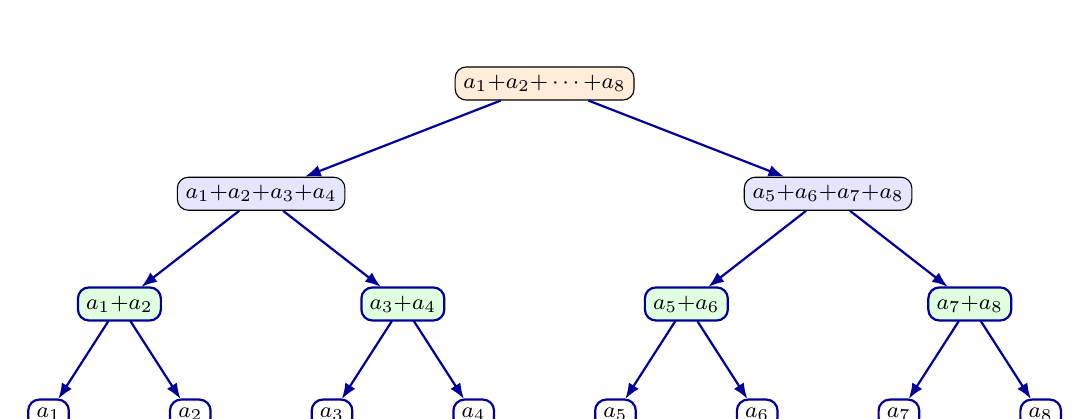
\begin{tikzpicture}[
  level distance=14mm,
  level 1/.style={sibling distance=72mm},
  level 2/.style={sibling distance=36mm},
  level 3/.style={sibling distance=18mm},
  every node/.style={draw, rounded corners, font=\footnotesize, inner sep=3pt},
  edge from parent/.style={draw, -{Latex[length=2mm]}, thick, blue!60!black}
]
\node[fill=orange!15] {\(a_1{+}a_2{+}\cdots{+}a_8\)}
  child {node[fill=blue!10] {\(a_1{+}a_2{+}a_3{+}a_4\)}
    child {node[fill=green!12] {\(a_1{+}a_2\)}
      child {node {\(a_1\)}}
      child {node {\(a_2\)}}}
    child {node[fill=green!12] {\(a_3{+}a_4\)}
      child {node {\(a_3\)}}
      child {node {\(a_4\)}}}}
  child {node[fill=blue!10] {\(a_5{+}a_6{+}a_7{+}a_8\)}
    child {node[fill=green!12] {\(a_5{+}a_6\)}
      child {node {\(a_5\)}}
      child {node {\(a_6\)}}}
    child {node[fill=green!12] {\(a_7{+}a_8\)}
      child {node {\(a_7\)}}
      child {node {\(a_8\)}}}};
\end{tikzpicture}
\end{center}

After the up-sweep, the in-place array $A$ holds:
\[
[a_1,\ a_1{+}a_2,\ a_3,\ a_1{+}a_2{+}a_3{+}a_4,\ a_5,\ a_5{+}a_6,\ a_7,\
 a_1{+}\cdots{+}a_8].
\]
The right children at each level contain useful partial sums; the left
children are left untouched, holding earlier intermediate sums.

\paragraph{Cost of the up-sweep.}
The number of additions at level $d$ is $n / 2^{d+1}$. Summing over
$d = 0, 1, \ldots, \log_2 n - 1$:
\[
W_{\mathrm{up}}(n) \;=\; \sum_{d=0}^{\log_2 n - 1} \frac{n}{2^{d+1}}
\;=\; \frac{n}{2} + \frac{n}{4} + \cdots + 1 \;=\; n - 1 \;=\; \Theta(n).
\]
There are $\log_2 n$ levels, each executable in parallel, giving depth
$\Theta(\log_2 n)$. \textbf{This phase is already work-efficient.}

\subsection{Phase 2: Down-Sweep}
\label{sec:downsweep}

The down-sweep traverses the tree from root to leaves, distributing
partial sums so that after the sweep, each leaf holds the prefix sum
that ends at it (inclusive variant) or just before it (exclusive variant).

\subsubsection{Inclusive Down-Sweep}
At each internal node, given a value passed in from above (initially the
total sum at the root), the rules are:
\begin{itemize}[leftmargin=*]
  \item The \textbf{left child} receives \emph{parent's value $-$ right child's value}
        (so it ends up with the sum of all leaves up to and including itself).
  \item The \textbf{right child} receives \emph{parent's value} (it already
        accumulates everything to its left from the up-sweep).
\end{itemize}

\begin{notebox}
\textbf{Why the inclusive rule works.} After the up-sweep, every right
child at a given level already holds the sum of its entire subtree. When
the parent passes its value (say $S$) down, the right child should hold
$S$ because $S$ is exactly the prefix ending at the rightmost leaf of
that subtree. The left child's new value must be $S$ minus the right
child's \emph{up-sweep} contribution, which gives the prefix ending at
the rightmost leaf of the left subtree.

This means the subtraction operation in the inclusive variant requires
the operator $\oplus$ to be \emph{invertible} (i.e., to have a defined
inverse). For addition this is fine, but for operators like $\max$ or
bitwise-OR there is no inverse, and the inclusive variant cannot be
computed this way. The exclusive variant (below) avoids this limitation
entirely and works for any associative operator.
\end{notebox}

\subsubsection{Exclusive Down-Sweep (the standard Blelloch variant)}
The more common \emph{exclusive scan} version is even cleaner. It uses the
following two rules, starting by placing the identity element ($0$ for
addition) at the root:
\begin{itemize}[leftmargin=*]
  \item \textbf{Left child} $\leftarrow$ parent's incoming value.
  \item \textbf{Right child} $\leftarrow$ parent's incoming value
        $+$ left child's up-sweep value.
\end{itemize}

\paragraph{Worked example (exclusive scan, $A = [3,1,7,0,4,1,6,3]$).}

After up-sweep, the tree (with root holding total $=25$) looks like:
\begin{center}
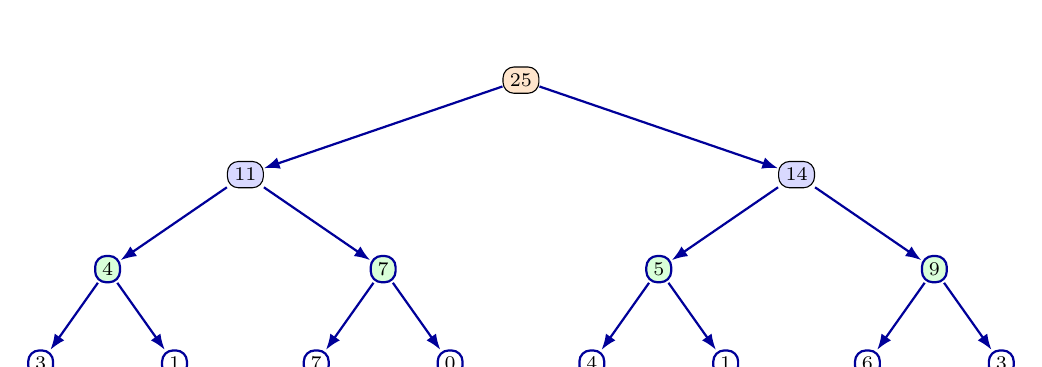
\begin{tikzpicture}[
  level distance=12mm,
  level 1/.style={sibling distance=70mm},
  level 2/.style={sibling distance=35mm},
  level 3/.style={sibling distance=17mm},
  every node/.style={draw, rounded corners, font=\scriptsize, inner sep=2.5pt},
  edge from parent/.style={draw, -{Latex[length=2mm]}, thick, blue!60!black}
]
\node[fill=orange!20] {25}
  child {node[fill=blue!15] {11}
    child {node[fill=green!15] {4}
      child {node {3}}
      child {node {1}}}
    child {node[fill=green!15] {7}
      child {node {7}}
      child {node {0}}}}
  child {node[fill=blue!15] {14}
    child {node[fill=green!15] {5}
      child {node {4}}
      child {node {1}}}
    child {node[fill=green!15] {9}
      child {node {6}}
      child {node {3}}}};
\end{tikzpicture}
\end{center}

\noindent For an exclusive scan we now \emph{set the root to 0} and apply
the down-sweep rules. The leaves end up containing the exclusive prefix
sums:
\[
[0,\ 3,\ 4,\ 11,\ 11,\ 15,\ 16,\ 22].
\]
(That is, leaf $i$ holds $A[1]+\cdots+A[i-1]$, with the convention that
the empty sum at $i=1$ is $0$.) An inclusive scan can be obtained from this
by shifting left and appending the total sum.

\paragraph{Down-sweep propagation, level by level.}
Starting from the root with value $0$:

\begin{center}
\begin{tabular}{l l}
\toprule
\textbf{Level} & \textbf{Values along this level (left $\to$ right)} \\
\midrule
Root (level 3) & $0$ \\
Level 2        & $0,\ 11$ \\
Level 1        & $0,\ 4,\ 11,\ 16$ \\
Level 0 (leaves)
              & $0,\ 3,\ 4,\ 11,\ 11,\ 15,\ 16,\ 22$ \\
\bottomrule
\end{tabular}
\end{center}

At each level, the left child inherits the parent's value while the
right child inherits parent's value plus the left child's
\emph{up-sweep} value. For instance, at level 2 the right child gets
$0 + 11 = 11$. At level 0 the entries
$\{0,3\}$ from the leftmost subtree are exactly the exclusive prefixes
of $\{3,1\}$.

\begin{notebox}
\textbf{Note (PRAM code, EREW).}
The down-sweep can be expressed in place as:
\begin{lstlisting}
A[n-1] <- 0   % identity
for d from log2(n) - 1 downto 0
    in parallel for i from 0 to n-1 by 2^(d+1)
        t                       <- A[i + 2^d - 1]      % save left subtree sum
        A[i + 2^d - 1]          <- A[i + 2^(d+1) - 1]  % left  <- parent
        A[i + 2^(d+1) - 1]      <- t + A[i + 2^(d+1) - 1]  % right <- parent + saved
\end{lstlisting}
This is exactly the algorithm given by Blelloch (1990).
\end{notebox}

\paragraph{Cost of the down-sweep.}
Each level performs the same number of operations as the corresponding
up-sweep level, so:
\[
W_{\mathrm{down}}(n) = \Theta(n), \qquad
T_{\mathrm{down}}(n) = \Theta(\log_2 n).
\]
Combined with the up-sweep:
\[
\boxed{\;W_{\mathrm{Blelloch}}(n) = \Theta(n), \qquad
T_{\mathrm{Blelloch}}(n) = \Theta(\log_2 n).\;}
\]

\subsection{PRAM Analysis: Hillis \& Steele vs. Blelloch}
\label{sec:pram-analysis}

We analyse both algorithms under the PRAM model, considering both the
\textbf{EREW} (Exclusive Read, Exclusive Write) and \textbf{CREW}
(Concurrent Read, Exclusive Write) variants.

\subsubsection{Hillis \& Steele}
At step $d$, every processor $i$ (with $i \ge 2^{d-1}$) reads
$A[i - 2^{d-1}]$ and its own current cell $A[i]$, then writes the
sum back to $A[i]$. Now consider two adjacent active processors, $i$
and $i + 2^{d-1}$: processor $i$ reads $A[i]$ as its source, while
processor $i + 2^{d-1}$ reads $A[(i+2^{d-1}) - 2^{d-1}] = A[i]$
simultaneously as its operand. Both processors therefore read the
\emph{same} memory cell concurrently. Since writes remain exclusive
(only processor $i$ writes to $A[i]$), Hillis \& Steele requires a
\textbf{CREW PRAM} --- concurrent reads, exclusive writes.

\begin{itemize}[leftmargin=*]
  \item \textbf{Steps:} $\lceil \log_2 n \rceil$.
  \item \textbf{Work:} $W(n) = O(n \log_2 n)$.
  \item \textbf{PRAM model:} \textbf{CREW} (concurrent reads on shared
        source cells; all writes exclusive).
  \item \textbf{Time on $p$ processors:}
        $T(n,p) = O\bigl(n \log_2 n / p + \log_2 n\bigr)$ assuming
        Brent's scheduling.
  \item \textbf{Efficiency:} $E_n = \Theta(1/\log_2 n) \to 0$.
\end{itemize}

\subsubsection{Blelloch}
The up-sweep and down-sweep both have a tree-shaped data dependence:
each parallel-for iteration at level $d$ touches a disjoint pair of
indices, so reads and writes are exclusive within a step. Blelloch's
algorithm therefore also runs on EREW PRAM.

For $p$ processors with $n > p$, each processor first sequentially
processes a chunk of size $n/p$, then participates in the tree of size
$p$. The total time is
\[
T_{\mathrm{Blelloch}}(n, p) \;=\; 2\!\left(\left\lceil \frac{n}{p} \right\rceil
+ \lceil \log_2 p \rceil\right) \;=\; O\!\left(\frac{n}{p} + \log_2 p\right).
\]
When $n / p \ge \log_2 p$, this gives \emph{optimal speedup} over the
sequential algorithm.

\subsubsection{Side-by-side comparison}

\begin{center}
\begin{tabular}{lll}
\toprule
\textbf{Property} & \textbf{Hillis \& Steele} & \textbf{Blelloch} \\
\midrule
Total work $W(n)$    & $\Theta(n \log_2 n)$        & $\Theta(n)$ \\
Depth $T_\infty(n)$  & $\Theta(\log_2 n)$          & $\Theta(\log_2 n)$ \\
PRAM model           & \textbf{CREW}               & EREW \\
Time on $p$ procs    & $O\!\left(\frac{n \log n}{p} + \log n\right)$
                                                   & $O\!\left(\frac{n}{p} + \log p\right)$ \\
Work-efficient?      & No                          & Yes \\
Number of passes     & 1 (left-to-right)           & 2 (up + down) \\
In-place?            & Yes                         & Yes \\
\bottomrule
\end{tabular}
\end{center}

\begin{keyideabox}
\textbf{Why Blelloch wins on work.} Hillis \& Steele activates roughly
$n$ processors at \emph{every} level, so its work is the depth times the
breadth: $n \log n$. Blelloch's tree halves the active processor count
at each level of the up-sweep ($n/2$, $n/4$, $n/8, \ldots$), and again
on the down-sweep, giving a geometric series that sums to $\Theta(n)$.
The depth stays the same; only redundant work is removed.
\end{keyideabox}

\begin{notebox}
\textbf{CREW vs.\ EREW.} As established above, Hillis \& Steele requires
\textbf{CREW PRAM} because adjacent processors concurrently read the same
source cell at every step. Blelloch is \textbf{EREW PRAM} because the
stride-based addressing ensures all reads and writes are to distinct
addresses within any parallel step. With concurrent reads (CREW), one can
additionally broadcast values cheaply, which lets certain
scan-with-bounded-operators variants achieve depth
$O(\log n / \log\log n)$ (Cole, 1986; Blelloch, 1990, ch.~4). Without
that machinery, $\Theta(\log n)$ is the standard depth bound.
\end{notebox}

% ----------------------------------------------------------
\section{Brent's Scheduling Theorem}
\label{sec:brents-theorem}

The analyses above repeatedly cite ``$T(n,p) = W/p + D$'' without formal
justification. This section states and explains the theorem that underlies
that bound.

\begin{keyideabox}
\textbf{Brent's Theorem (1974).} Let a parallel algorithm have total work
$W$ (number of operations) and depth $D$ (longest chain of dependencies).
Then on $p$ processors, the algorithm can be scheduled to finish in time
\[
T(n,p) \;\le\; \left\lfloor \frac{W}{p} \right\rfloor + D.
\]
\end{keyideabox}

\noindent\textbf{Proof sketch.} Consider the computation as a DAG with $W$
nodes (operations) and depth $D$. A \emph{greedy} scheduler at each step
picks as many ready operations as possible and assigns them to idle
processors. At step $t$, let $w_t$ be the number of operations scheduled.
Two cases:
\begin{enumerate}[leftmargin=*]
  \item $w_t = p$: all processors are busy.
  \item $w_t < p$: some processors are idle, meaning all remaining
        operations depend on work in progress. This forces at least one
        step along the critical path, so this situation can recur at most
        $D$ times total.
\end{enumerate}
Let $T_1$ be the total number of steps in case (1) and $T_2$ the steps in
case (2). The total work done in case-1 steps is at least $p T_1$, so
$T_1 \le W / p$. By the critical-path argument, $T_2 \le D$. Since every
step is either case (1) or case (2):
\[
T(n,p) = T_1 + T_2 \le \frac{W}{p} + D.
\]

\paragraph{Applying Brent's Theorem to our algorithms.}
\begin{center}
\begin{tabular}{lllll}
\toprule
\textbf{Algorithm} & $W$ & $D$ & $T(n,p)$ bound \\
\midrule
Sequential         & $\Theta(n)$         & $\Theta(n)$ & $\Theta(n)$ (single proc.) \\
Hillis \& Steele   & $\Theta(n \log n)$  & $\Theta(\log n)$
                   & $O(n \log n / p + \log n)$ \\
Blelloch           & $\Theta(n)$         & $\Theta(\log n)$
                   & $O(n/p + \log n)$ \\
\bottomrule
\end{tabular}
\end{center}

\begin{notebox}
\textbf{Why the Blelloch depth term is $\log n$ here but $\log p$ elsewhere.}
Brent's Theorem is applied above using the algorithm's intrinsic depth $D$
when scheduled on $n$ dedicated processors: for Blelloch this is
$2\lceil\log_2 n\rceil = \Theta(\log n)$. This gives the bound
$T(n,p) \le n/p + \log n$.

In Section~\ref{sec:pram-analysis}, we instead use a refined
\emph{chunk\,+\,tree} analysis: each of the $p$ processors first
handles $n/p$ elements sequentially (sequential scan of its chunk),
then the $p$ partial results are combined via a $p$-leaf Blelloch tree
of depth $\log_2 p$. This gives the tighter formula
$T_{\mathrm{Blelloch}}(n,p) = O(n/p + \log_2 p)$, which is strictly
better than $O(n/p + \log n)$ whenever $p < n$. The comparison table
in Section~\ref{sec:pram-analysis} uses the tighter $\log p$ bound;
the table above shows the direct Brent application using the algorithm's
raw depth $\log n$.
\end{notebox}

\noindent Blelloch achieves \textbf{optimal speedup} when $n/p \gg \log n$:
under that condition $T \approx n/p$, which is the best any algorithm using
$p$ processors can do to process $n$ inputs. Hillis \& Steele requires
$n \log n / p \gg \log n$, i.e.\ $n \gg p$, to be competitive --- and even
then wastes a $\log n$ factor compared to Blelloch.

% ----------------------------------------------------------
\section{Side-by-Side Trace: Hillis \& Steele vs.\ Blelloch}
\label{sec:sidebyside}

The PRAM comparison table in Section~\ref{sec:pram-analysis} gives
\emph{asymptotic} numbers. This section makes those numbers concrete by
running \textbf{both algorithms on the same 8-element array} and
counting every single addition. The goal is to see, in exact arithmetic,
why Blelloch's work count stays near $2n$ while Hillis \& Steele's
climbs toward $n \log_2 n$.

We use the array
\[
A \;=\; [\,6,\ 2,\ 5,\ 1,\ 4,\ 3,\ 7,\ 0\,]
\]
whose true inclusive prefix sums are
$[\,6,\ 8,\ 13,\ 14,\ 18,\ 21,\ 28,\ 28\,]$.

\subsection{Hillis \& Steele Full Trace}

At step $d$, every processor $i \ge 2^{d-1}$ adds $A[i - 2^{d-1}]$
to its running value. Processors with $i < 2^{d-1}$ are idle.
Idle positions are shown in plain text; updated positions are
\textbf{bold}.

\begin{center}
\renewcommand{\arraystretch}{1.25}
\begin{tabular}{lccccccccr}
\toprule
\textbf{Step} & [0] & [1] & [2] & [3] & [4] & [5] & [6] & [7]
              & \textbf{Adds} \\
\midrule
Input         & 6 & 2 & 5 & 1 & 4 & 3 & 7 & 0 & --- \\
$d=1$ (+1)    & 6 & \textbf{8} & \textbf{7} & \textbf{6} &
                \textbf{5} & \textbf{7} & \textbf{10} & \textbf{7} & 7 \\
$d=2$ (+2)    & 6 & 8 & \textbf{13} & \textbf{14} &
                \textbf{12} & \textbf{13} & \textbf{15} & \textbf{17} & 6 \\
$d=3$ (+4)    & 6 & 8 & 13 & 14 &
                \textbf{18} & \textbf{21} & \textbf{28} & \textbf{28} & 4 \\
\midrule
\multicolumn{9}{r}{\textbf{Total additions}} & \textbf{17} \\
\bottomrule
\end{tabular}
\end{center}

\noindent The final row matches the expected prefix sums. \checkmark

\paragraph{Work count, step by step.}
At step $d$, the number of active processors is $n - 2^{d-1}$:
\[
d=1:\; 8-1=7, \qquad d=2:\; 8-2=6, \qquad d=3:\; 8-4=4.
\]
Total $= 7 + 6 + 4 = \mathbf{17}$ additions.
Sequential algorithm needs exactly $n-1 = 7$ additions.
Hillis \& Steele does $\mathbf{17/7 \approx 2.4\times}$ more work.

\begin{notebox}
\textbf{General formula.}
$W_{\mathrm{HS}}(n)
= \sum_{d=1}^{\log_2 n}(n - 2^{d-1})
= n\log_2 n - (n-1)
= \Theta(n\log_2 n)$.
For $n = 8$: $8 \cdot 3 - 7 = 17$. \checkmark
\end{notebox}

\subsection{Blelloch Full Trace}

\subsubsection*{Phase 1: Up-Sweep}

At level $d$ (stride $s = 2^{d+1}$), every right element of each
stride-$s$ block absorbs the left element immediately $s/2$ positions
to its left. Left elements are unchanged.

\begin{center}
\renewcommand{\arraystretch}{1.25}
\begin{tabular}{lccccccccr}
\toprule
\textbf{Level} & [0] & [1] & [2] & [3] & [4] & [5] & [6] & [7]
               & \textbf{Adds} \\
\midrule
Start          & 6 & 2 & 5 & 1 & 4 & 3 & 7 & 0 & --- \\
0 (stride 2)   & 6 & \textbf{8} & 5 & \textbf{6} & 4 & \textbf{7} & 7 & \textbf{7} & 4 \\
1 (stride 4)   & 6 & 8 & 5 & \textbf{14} & 4 & 7 & 7 & \textbf{14} & 2 \\
2 (stride 8)   & 6 & 8 & 5 & 14 & 4 & 7 & 7 & \textbf{28} & 1 \\
\midrule
\multicolumn{9}{r}{\textbf{Subtotal (up-sweep)}} & \textbf{7} \\
\bottomrule
\end{tabular}
\end{center}

After the up-sweep, $A[7] = 28$ (total sum). \checkmark

\subsubsection*{Phase 2: Exclusive Down-Sweep}

Set $A[7] \leftarrow 0$. At each level (stride halves from $n$ down to
$2$), each pair applies: left child $\leftarrow$ parent's value;
right child $\leftarrow$ parent's value + left child's up-sweep value.

\begin{center}
\renewcommand{\arraystretch}{1.25}
\begin{tabular}{lccccccccr}
\toprule
\textbf{Level} & [0] & [1] & [2] & [3] & [4] & [5] & [6] & [7]
               & \textbf{Adds} \\
\midrule
Set root $\leftarrow 0$ & 6 & 8 & 5 & 14 & 4 & 7 & 7 & \textbf{0} & --- \\
2 (stride 8)   & 6 & 8 & 5 & \textbf{0} & 4 & 7 & 7 & \textbf{14} & 1 \\
1 (stride 4)   & 6 & \textbf{0} & 5 & \textbf{8} & 4 & \textbf{14} & 7 & \textbf{21} & 2 \\
0 (stride 2)   & \textbf{0} & \textbf{6} & \textbf{8} & \textbf{13} &
                 \textbf{14} & \textbf{18} & \textbf{21} & \textbf{28} & 4 \\
\midrule
\multicolumn{9}{r}{\textbf{Subtotal (down-sweep)}} & \textbf{7} \\
\bottomrule
\end{tabular}
\end{center}

Final exclusive prefix sum:
$[\,0,\ 6,\ 8,\ 13,\ 14,\ 18,\ 21,\ 28\,]$.
(Entry $i$ = sum of all elements \emph{before} position $i$.) \checkmark

\paragraph{Total Blelloch work.}
Up-sweep: $4 + 2 + 1 = 7$.
Down-sweep: $1 + 2 + 4 = 7$.
Grand total $= \mathbf{14}$ additions $= 2(n-1)$ for $n=8$.
Compare to sequential $n-1=7$: Blelloch does only
$\mathbf{2\times}$ the sequential work --- a constant factor.

\subsection{Work Comparison Summary}

\begin{center}
\renewcommand{\arraystretch}{1.3}
\begin{tabular}{lccc}
\toprule
\textbf{Algorithm} & \textbf{Additions ($n=8$)} & \textbf{Depth (steps)}
                   & \textbf{Work-efficient?} \\
\midrule
Sequential         & 7                   & 7 (no parallelism)    & --- \\
Hillis \& Steele   & 17                  & 3 ($\log_2 8$)        & No \\
Blelloch           & 14                  & 6 ($2\log_2 8$)       & \textbf{Yes} \\
\bottomrule
\end{tabular}
\end{center}

\begin{keyideabox}
\textbf{The key trade-off, made concrete.}
Hillis \& Steele achieves its $O(\log_2 n)$ depth by keeping \emph{all}
processors active at every level --- it pays for speed with extra work.
Blelloch achieves the same depth across two phases by halving the number
of active processors at each level: it does $n/2$ additions at level 0,
$n/4$ at level 1, and so on, with the down-sweep mirroring the up-sweep.
The total telescopes to $2(n-1)$, which is just $2\times$ the sequential
cost regardless of $n$. The depth is $2\log_2 n$ (not $\log_2 n$ as in
H\&S), but this constant factor is irrelevant asymptotically and
negligible in practice compared to the $\log_2 n$ work overhead of H\&S.
\end{keyideabox}

% ----------------------------------------------------------
\section{Parallel Radix Sort}
\label{sec:radix-sort}

\textbf{Radix sort} is a non-comparison-based sorting algorithm. Rather
than comparing keys to one another, it processes keys digit by digit,
using a stable bucket-sort at each digit position. Its real-world uses
are everywhere:

\begin{itemize}[leftmargin=*]
  \item \textbf{Apache Spark and Apache Flink:} radix sort underlies
        \emph{group-by} and \emph{join} operations on huge datasets.
  \item \textbf{IP routing:} sorting and searching massive IP tables for
        packet routing.
  \item \textbf{DNA sequencing:} mapping short DNA reads to a reference
        genome.
\end{itemize}

\subsection{Sequential Radix Sort}
Let $A = [a_1, a_2, \ldots, a_n]$ with each $a_i$ a $d$-digit number in
some radix $k$ (say $k = 10$ for decimal, or $k = 2^8 = 256$ for
byte-radix). Sequential LSD (least-significant-digit) radix sort
processes one digit at a time, from least to most significant, using a
stable counting sort. Each pass has three phases.

\paragraph{Step 1: Histogram (count) construction.}
Build an array \texttt{count[0..k-1]} where \texttt{count[v]} is the
number of elements whose current digit equals $v$.

\paragraph{Step 2: Prefix sum.}
Replace \texttt{count} with its \emph{exclusive} prefix sum, giving
\texttt{count\_prefix[v]} = the starting output index for the bucket
of value $v$.

\paragraph{Step 3: Scatter.}
Walk the input left-to-right; place each element at its bucket's current
write pointer (read from \texttt{count\_prefix}) and increment that
pointer.

\subsection{Worked Example}
\label{sec:radix-example}
Let $A = [170,\ 45,\ 75,\ 90,\ 802,\ 24,\ 2,\ 66]$ with radix $k=10$.

\subsubsection*{Pass 1: sort by units digit}

\textbf{Step 1 (histogram).} The units digits are
$[0, 5, 5, 0, 2, 4, 2, 6]$, so:
\[
\texttt{count} \;=\; [\,2,\ 0,\ 2,\ 0,\ 1,\ 2,\ 1,\ 0,\ 0,\ 0\,].
\]

\textbf{Step 2 (exclusive prefix sum on count).}
\[
\texttt{count\_prefix} \;=\; [\,0,\ 2,\ 2,\ 4,\ 4,\ 5,\ 7,\ 8,\ 8,\ 8\,].
\]
Reading off \texttt{count\_prefix} as a table:
\begin{center}
\begin{tabular}{ccc}
\toprule
\textbf{digit $d$} & \textbf{count[d]} & \textbf{start index} \\
\midrule
0 & 2 & 0 \\
1 & 0 & 2 \\
2 & 2 & 2 \\
3 & 0 & 4 \\
4 & 1 & 4 \\
5 & 2 & 5 \\
6 & 1 & 7 \\
7 & 0 & 8 \\
8 & 0 & 8 \\
9 & 0 & 8 \\
\bottomrule
\end{tabular}
\end{center}

\textbf{Step 3 (scatter).} Walk over $A$. Each element looks up its
bucket's start index, writes itself there, and advances the pointer:
\begin{center}
\begin{tabular}{lcl}
\toprule
\textbf{Element} & \textbf{Digit} & \textbf{Output index} \\
\midrule
170 & 0 & 0 \\
45  & 5 & 5 \\
75  & 5 & 6 \\
90  & 0 & 1 \\
802 & 2 & 2 \\
24  & 4 & 4 \\
2   & 2 & 3 \\
66  & 6 & 7 \\
\bottomrule
\end{tabular}
\end{center}
After the scatter:
\[
A \;=\; [\,170,\ 90,\ 802,\ 2,\ 24,\ 45,\ 75,\ 66\,].
\]

\subsubsection*{Pass 2: sort by tens digit}
\[
A \;=\; [\,802,\ 2,\ 24,\ 45,\ 66,\ 170,\ 75,\ 90\,].
\]

\subsubsection*{Pass 3: sort by hundreds digit}
\[
A \;=\; [\,2,\ 24,\ 45,\ 66,\ 75,\ 90,\ 170,\ 802\,].
\]
The array is now sorted. Each pass is $O(n + k)$, and there are $d$
passes, so the sequential complexity is $\Theta(d \cdot (n + k))$. With
$k = O(n)$ this simplifies to $\Theta(d \cdot n)$.

\subsection{Parallel Radix Sort}
\label{sec:parallel-radix}

We now parallelise each of the three steps using $p$ processors that
each own a contiguous chunk of the input of size $n/p$. To make every
cost concrete, we will run a small worked example alongside the
analysis.

\begin{examplebox}
\textbf{Running example.} Take $n = 8$ keys, $p = 4$ processors, radix
$k = 4$, and the array
\[
A \;=\; [\,3,\ 1,\ 0,\ 2,\ 3,\ 0,\ 1,\ 2\,].
\]
Each processor owns two consecutive elements:
\begin{center}
\begin{tabular}{cc}
\toprule
\textbf{Processor} & \textbf{Owns} \\
\midrule
$P_0$ & $[3,\ 1]$ \\
$P_1$ & $[0,\ 2]$ \\
$P_2$ & $[3,\ 0]$ \\
$P_3$ & $[1,\ 2]$ \\
\bottomrule
\end{tabular}
\end{center}
We will sort by the only digit (one pass suffices because all keys are
single-digit). Final answer expected: $[0,0,1,1,2,2,3,3]$.
\end{examplebox}

\subsubsection{Step 1 --- Parallel Histogram}

\paragraph{1a. Local counting (embarrassingly parallel).}
Each processor scans its own $n/p$ elements and builds a \emph{private}
length-$k$ histogram, with no communication.
For our example:
\begin{center}
\begin{tabular}{c|cccc|c}
\toprule
\textbf{Processor} & \textbf{cnt[0]} & \textbf{cnt[1]} & \textbf{cnt[2]} & \textbf{cnt[3]}
                   & \textbf{Reasoning} \\
\midrule
$P_0$ & 0 & 1 & 0 & 1 & owns $[3,1]$: one ``1'', one ``3'' \\
$P_1$ & 1 & 0 & 1 & 0 & owns $[0,2]$ \\
$P_2$ & 1 & 0 & 0 & 1 & owns $[3,0]$ \\
$P_3$ & 0 & 1 & 1 & 0 & owns $[1,2]$ \\
\bottomrule
\end{tabular}
\end{center}
Each processor reads $n/p = 2$ elements and performs one increment per
element on its \emph{private} array of size $k$. There are no shared
writes, so this phase is truly embarrassingly parallel.

\begin{keyideabox}
\textbf{Why local counting is $\Theta(n/p)$.} Every processor does
exactly $n/p$ reads and $n/p$ increments on memory it alone owns. No
synchronisation, no contention. With $p$ processors running
simultaneously, the wall-clock time is the time of one
processor:~$\Theta(n/p)$.
\end{keyideabox}

\paragraph{1b. Combining local histograms (the source of $k\log_2 p$).}
The local histograms now form a $p \times k$ matrix; the global
histogram is the column-wise sum. We use a tree reduction across
processors --- $\log_2 p$ rounds of pairing, where in each round each
active processor receives a partner's histogram and adds it to its own,
\emph{element by element}.

For our example ($p=4$, $k=4$, so $\log_2 p = 2$ rounds):
\begin{center}
\begin{tabular}{l|cccc|l}
\toprule
& \textbf{[0]} & \textbf{[1]} & \textbf{[2]} & \textbf{[3]} & \textbf{Notes} \\
\midrule
\textbf{Round 0:} $P_0 \leftarrow P_0 + P_1$ & 1 & 1 & 1 & 1 & $P_0$: 4 adds \\
\quad\quad\quad\;\; $P_2 \leftarrow P_2 + P_3$ & 1 & 1 & 1 & 1 & $P_2$: 4 adds \\
\midrule
\textbf{Round 1:} $P_0 \leftarrow P_0 + P_2$ & 2 & 2 & 2 & 2 & $P_0$: 4 adds \\
\bottomrule
\end{tabular}
\end{center}
After two rounds, $P_0$ holds the global histogram $[2, 2, 2, 2]$.

\begin{keyideabox}
\textbf{Where does $k \log_2 p$ come from?} At each of the $\log_2 p$
rounds, each \emph{active} processor must add a partner's entire
size-$k$ histogram to its own. That is $k$ scalar additions per active
processor per round. Since rounds are sequential (round $r+1$ depends on
round $r$), the wall-clock time is the sum over rounds:
\[
\underbrace{O(k)}_{\text{round 1}} + \underbrace{O(k)}_{\text{round 2}}
+ \cdots + \underbrace{O(k)}_{\text{round } \log_2 p}
\;=\; O(k \cdot \log_2 p).
\]
The factor of $k$ comes from the size of the object being communicated
and added at each step; the factor of $\log_2 p$ comes from the depth
of the reduction tree over $p$ processors.
\end{keyideabox}

\subsubsection{Step 2 --- Parallel Prefix Sum on the Global Histogram}
The exclusive prefix-sum on the length-$k$ global histogram is exactly
the scan problem of Section~\ref{sec:blelloch}. For our example:
\[
\texttt{count} = [2,2,2,2]
\;\longrightarrow\;
\texttt{count\_prefix} = [0,\ 2,\ 4,\ 6].
\]
This tells us where each digit's bucket starts in the output:
digit $0$ at index $0$, digit $1$ at index $2$, digit $2$ at index $4$,
digit $3$ at index $6$.

Using Blelloch on $p$ processors gives time
$\Theta(k/p + \log_2 p)$. Because $k$ is typically small ($k=10$ for
decimal, $k=256$ for byte-radix), this step is almost always dominated
by the histogram-combine cost above.

\subsubsection{Step 3 --- Parallel Scatter}

The naive sequential scatter has a write-after-write race: two
processors might both try to write to bucket $v$, collide on its single
write pointer, and overwrite each other. We avoid this by computing
\emph{per-processor offsets} so that each processor knows the unique
output position of every element it owns.

\paragraph{3a. Per-processor bucket offsets.}
For each digit $v$, processor $i$'s elements with digit $v$ should
appear in the output \emph{after} all such elements owned by processors
$0,1,\ldots,i-1$. We therefore need the column-wise \emph{exclusive
prefix sum} of the $p \times k$ local-histogram matrix. For our running
example:
\begin{center}
\begin{tabular}{c|cccc|c|cccc}
\toprule
& \multicolumn{4}{c|}{\textbf{Local histograms}}
& & \multicolumn{4}{c}{\textbf{Column prefix sums (excl.)}} \\
\textbf{Proc} & \textbf{[0]} & \textbf{[1]} & \textbf{[2]} & \textbf{[3]}
& & \textbf{[0]} & \textbf{[1]} & \textbf{[2]} & \textbf{[3]} \\
\midrule
$P_0$ & 0 & 1 & 0 & 1 & & 0 & 0 & 0 & 0 \\
$P_1$ & 1 & 0 & 1 & 0 & & 0 & 1 & 0 & 1 \\
$P_2$ & 1 & 0 & 0 & 1 & & 1 & 1 & 1 & 1 \\
$P_3$ & 0 & 1 & 1 & 0 & & 2 & 1 & 1 & 2 \\
\bottomrule
\end{tabular}
\end{center}
Adding the global \texttt{count\_prefix} (the bucket starts) to these
column offsets gives, for each (processor, digit) pair, the exact output
position where that processor should start writing its digit-$v$
elements:
\begin{center}
\begin{tabular}{c|cccc}
\toprule
\textbf{Processor} & \textbf{digit 0} & \textbf{digit 1} & \textbf{digit 2} & \textbf{digit 3} \\
& (bucket start 0) & (bucket start 2) & (bucket start 4) & (bucket start 6) \\
\midrule
$P_0$ & $0+0 = 0$ & $2+0 = 2$ & $4+0 = 4$ & $6+0 = 6$ \\
$P_1$ & $0+0 = 0$ & $2+1 = 3$ & $4+0 = 4$ & $6+1 = 7$ \\
$P_2$ & $0+1 = 1$ & $2+1 = 3$ & $4+1 = 5$ & $6+1 = 7$ \\
$P_3$ & $0+2 = 2$ & $2+1 = 3$ & $4+1 = 5$ & $6+2 = 8$ \\
\bottomrule
\end{tabular}
\end{center}
Computing all $k$ column-wise prefix sums via a tree-style scan over
$p$ processors costs $O(k \log_2 p)$ --- the same analysis as the
combine step.

\paragraph{3b. The actual scatter (back to $\Theta(n/p)$).}
Now every processor knows, for each of its $n/p$ elements, exactly which
output position to write to. Each processor walks through its own chunk
and emits elements into the precomputed positions:
\begin{center}
\begin{tabular}{c|c|c|c}
\toprule
\textbf{Processor} & \textbf{Element (digit)} & \textbf{Output position} & \textbf{Effect} \\
\midrule
$P_0$ & $3$ (digit 3) & $6$ & $\text{out}[6] = 3$ \\
$P_0$ & $1$ (digit 1) & $2$ & $\text{out}[2] = 1$ \\
$P_1$ & $0$ (digit 0) & $0$ & $\text{out}[0] = 0$ \\
$P_1$ & $2$ (digit 2) & $4$ & $\text{out}[4] = 2$ \\
$P_2$ & $3$ (digit 3) & $7$ & $\text{out}[7] = 3$ \\
$P_2$ & $0$ (digit 0) & $1$ & $\text{out}[1] = 0$ \\
$P_3$ & $1$ (digit 1) & $3$ & $\text{out}[3] = 1$ \\
$P_3$ & $2$ (digit 2) & $5$ & $\text{out}[5] = 2$ \\
\bottomrule
\end{tabular}
\end{center}
Final output: $[0,\ 0,\ 1,\ 1,\ 2,\ 2,\ 3,\ 3]$. Sorted, as required.

\begin{keyideabox}
\textbf{Why the scatter is $\Theta(n/p)$, not slower.}
\begin{enumerate}[leftmargin=*]
  \item \emph{No two processors write to the same output position.}
        The offsets were computed precisely so each (processor, digit)
        pair owns a distinct, contiguous run of output slots. There is
        no contention, no atomic, no lock --- just plain writes.
  \item \emph{Each processor performs exactly $n/p$ writes,} one per
        element it owns. There is no extra traversal of the input
        array, no merging, no comparison.
  \item \emph{Per-element work is constant:} look up the bucket for the
        element's digit, write the element to the next available slot
        in that bucket, increment the local pointer.
\end{enumerate}
With $p$ processors running in parallel, each finishing $n/p$ writes
independently, total time is $\Theta(n/p)$.
\end{keyideabox}

\begin{notebox}
\textbf{Where the racing would have been.} If we had skipped step 3a
and just shared one global write-pointer per bucket, every processor
with a digit-$v$ element would race on the same pointer. The fix
(atomics) serialises updates per bucket; in the worst case, all $n/p$
elements per processor target the same bucket and atomic contention
turns scatter into $\Theta(n)$ --- losing the parallelism entirely.
The prefix-sum-based offset computation completely eliminates this
race \emph{ahead of time}.
\end{notebox}

\subsection{Stability of Parallel Radix Sort}
\label{sec:stability}

A sorting pass is \emph{stable} if elements that share the same key value
appear in the output in the same relative order as they appeared in the input.
Stability is not merely a cosmetic property for radix sort: it is
\textbf{essential for correctness}. After sorting by the units digit, the
order among elements sharing the same units digit encodes information about
their original positions. The next pass (tens digit) must preserve that order
within each bucket; otherwise the sorting invariant breaks down.

\paragraph{Why the parallel scatter is stable.}
Each processor $P_i$ processes its $n/p$ elements \emph{left-to-right} in
input order. For a given digit $v$, $P_i$'s column offset (computed in step
3a) gives the starting slot for $P_i$'s digit-$v$ elements. Because $P_i$
iterates its chunk in order and writes to consecutive slots starting at that
offset, elements from $P_i$ with digit $v$ appear in the output in exactly
their input order. Because processors are assigned to contiguous chunks of
the input, all elements from $P_0$'s chunk precede all elements from $P_1$'s
chunk in the output, and so on. This gives global stability: for any two
elements $x$ and $y$ with the same digit, if $x$ appeared before $y$ in the
input, then $x$ appears before $y$ in the output.

\begin{pitfallbox}
\textbf{Common mistake: chunk assignment breaks stability.} If processors
are assigned \emph{non-contiguous} stripes of the input (e.g.\ $P_i$ owns
all elements at positions $\equiv i \pmod{p}$), the offset computation still
works, but the output order within a bucket follows the interleaved pattern
of the stripe, not the original input order. The sort may still produce a
sorted output on the last pass, but intermediate passes lose stability. Using
contiguous chunks is the correct choice.
\end{pitfallbox}

\subsection{PRAM Complexity Analysis}
\label{sec:radix-pram}

Putting the three steps together for one digit pass:
\[
T_{\mathrm{pass}}(n,p,k) \;=\;
\underbrace{\Theta\!\left(\tfrac{n}{p}\right)}_{\substack{\text{local count}\\ \text{(step 1a)}}}
\;+\;
\underbrace{\Theta(k \log_2 p)}_{\substack{\text{combine + scan + offsets}\\ \text{(steps 1b, 2, 3a)}}}
\;+\;
\underbrace{\Theta\!\left(\tfrac{n}{p}\right)}_{\substack{\text{scatter}\\ \text{(step 3b)}}}
\;=\;
\Theta\!\left(\tfrac{n}{p} + k \log_2 p\right).
\]
There are $d$ passes (one per digit position), so:
\[
\boxed{\;T_{\mathrm{radix}}(n, p, k, d) \;=\;
\Theta\!\left(d \cdot \left(\tfrac{n}{p} + k \log_2 p\right)\right).\;}
\]

\paragraph{Decoding the formula, term by term.}
\begin{itemize}[leftmargin=*]
  \item The $n/p$ term is the \textbf{data-movement cost}: every key
        must be read once (during local counting) and written once
        (during scatter). With $p$ processors sharing the work, each
        handles $n/p$ keys.
  \item The $k \log_2 p$ term is the \textbf{coordination cost} between
        processors. The factor $k$ is the size of the histogram object
        that has to traverse the reduction/scan tree; the factor
        $\log_2 p$ is the depth of that tree. Bigger radix $\Rightarrow$
        bigger histogram $\Rightarrow$ more coordination work per tree
        level. More processors $\Rightarrow$ taller tree.
  \item The leading $d$ counts how many digit positions need to be
        processed (e.g.\ $d = 4$ for 32-bit keys at $k = 256$).
\end{itemize}

\paragraph{Asymptotic regimes.}
\begin{itemize}[leftmargin=*]
  \item \textbf{Big-data regime} ($n/p \gg k \log_2 p$): the bound
        collapses to $\Theta(d \cdot n / p)$, an optimal $p$-fold
        speedup over the sequential $\Theta(d \cdot n)$.
  \item \textbf{Coordination-bound regime} ($n/p$ comparable to or
        smaller than $k \log_2 p$): the histogram-combine dominates.
        Remedies are to shrink $k$, use fewer processors, or merge
        small chunks before sorting.
\end{itemize}

\begin{notebox}
\textbf{Stability matters.} For multi-pass radix sort to be correct,
each digit pass must be \emph{stable}: it must preserve the relative
order of elements that share the same digit value. The scatter step
above is stable because each processor writes its elements in input
order into its bucket region, and processors with earlier chunks own
earlier output positions.
\end{notebox}

\paragraph{Choosing the radix $k$ optimally.}
An interesting engineering question is: what is the best choice of $k$
for a given $n$ and $p$? The time per pass is $\Theta(n/p + k \log_2 p)$
and there are $d = B / \log_2 k$ passes for $B$-bit keys. The total time
is proportional to
\[
\frac{B}{\log_2 k} \cdot \left(\frac{n}{p} + k \log_2 p\right).
\]
Setting the derivative with respect to $k$ to zero (treating $k$ as
continuous) gives the optimal $k^* \approx n / (p \log_2 p)$. In
practice, $k$ is usually a power of two for bit-manipulation convenience,
so one picks the nearest power of two to $k^*$. For large $n/p$ (many
elements per processor) a larger $k$ is preferred because it reduces the
number of passes, while for small $n/p$ a smaller $k$ is better because
the coordination cost dominates.

% ----------------------------------------------------------
\section{Problems and Solutions}
\label{sec:problems}

\subsection{Problem 1: Trace Blelloch's exclusive scan}
Given $A = [4, 7, 1, 0, 5, 2, 6, 4]$, perform Blelloch's exclusive
$+$-scan and show the contents of the array after the up-sweep, after
zeroing the root, and after the down-sweep.

\paragraph{Solution.}
\textbf{Up-sweep.}
\begin{itemize}[leftmargin=*]
  \item Level 0: $A = [4, 11, 1, 1, 5, 7, 6, 10]$
  \item Level 1: $A = [4, 11, 1, 12, 5, 7, 6, 17]$
  \item Level 2: $A = [4, 11, 1, 12, 5, 7, 6, 29]$
\end{itemize}
\textbf{Zero the root:} $A[7] \leftarrow 0$, giving
$A = [4, 11, 1, 12, 5, 7, 6, 0]$.\\
\textbf{Down-sweep.} Following the rules left $\leftarrow$ parent and
right $\leftarrow$ parent + saved-left, we obtain the exclusive prefix
sums:
\[
A \;=\; [\,0,\ 4,\ 11,\ 12,\ 12,\ 17,\ 19,\ 25\,].
\]
You can verify each entry against $\sum_{j<i} A_{\mathrm{orig}}[j]$.

\subsection{Problem 2: Hillis \& Steele on a non-power-of-two array}
What happens if we run Hillis \& Steele on an array of length $n$ that
is \emph{not} a power of two? How many steps does the algorithm need?

\paragraph{Solution.}
The algorithm still works correctly. At step $d$, processor $i$ adds
$A[i - 2^{d-1}]$ to its current value if that index is $\ge 0$;
otherwise it does nothing. The number of steps is
$\lceil \log_2 n \rceil$. After this many passes, the doubling window
exceeds $n$, so each cell has accumulated all preceding values. The
only inefficiency is that the last few processors do nothing on the
late steps, which slightly reduces utilisation but does not change the
asymptotic bounds.

\subsection{Problem 3: Radix-sort histogram race}
Suppose two threads share a single global histogram and both increment
\texttt{count[v]} for the same digit $v$ at the same time, without
synchronisation. What goes wrong, and how do we fix it?

\paragraph{Solution.}
This is a classic write-after-write race. The increment
\texttt{count[v]++} is a read-modify-write; if both threads read $c$
at the same time, both will write $c+1$, losing one of the increments.
The two standard fixes:
\begin{enumerate}[leftmargin=*]
  \item \textbf{Atomic increments:} replace \texttt{count[v]++} with
        \texttt{atomicAdd(\&count[v], 1)}. This serialises updates to
        the same bucket and is correct, but slow under contention.
  \item \textbf{Per-thread private histograms} (the parallel-radix
        approach in Section~\ref{sec:parallel-radix}): each thread
        builds its own \texttt{count} privately, then a tree-reduction
        merges them. No atomics, no contention.
\end{enumerate}

% ----------------------------------------------------------
\section{Key Takeaways}
\begin{itemize}[leftmargin=*]
  \item Although prefix sum looks sequential, an associative operator
        is enough to admit $O(\log_2 n)$-depth parallel algorithms.
  \item Hillis \& Steele is conceptually simple, $O(\log_2 n)$ depth,
        but does $\Theta(n \log_2 n)$ work --- not work-efficient.
  \item Blelloch's two-phase up-sweep / down-sweep does $\Theta(n)$
        work at the same depth, so it is work-efficient.
  \item Hillis \& Steele requires \textbf{CREW PRAM}: at each step,
        two adjacent processors read the same source cell simultaneously.
        Blelloch's stride-based addressing ensures all reads and writes
        are to distinct addresses, so it runs on the weaker \textbf{EREW PRAM}.
        On $p$ processors with $n > p$, Blelloch achieves optimal
        $O(n/p + \log_2 p)$ time.
  \item Brent's Theorem provides the formal bridge from work $W$ and
        depth $D$ to the time on $p$ processors: $T(n,p) \le W/p + D$.
        Work-efficient algorithms benefit most from this bound.
  \item Parallel radix sort decomposes into three steps:
        embarrassingly-parallel histogram, parallel prefix sum, and
        carefully-coordinated parallel scatter.
  \item The scatter step is stable when processors own contiguous input
        chunks and write their elements in order, which is necessary
        for multi-pass radix sort to be correct.
  \item Total time of parallel radix sort is
        $\Theta(d (n/p + k \log_2 p))$, giving optimal speedup over
        sequential when $n/p \gg k \log_2 p$.
\end{itemize}

% ----------------------------------------------------------
\section{Exercises and Solutions}
\label{sec:exercises}

\begin{exercisebox}
\textbf{Exercise 6.1.} State the formal definition of the
all-prefix-sums operation. What property of the operator $\oplus$ is
required for parallelisation, and why?

\medskip
\textbf{Solution.} Given a binary associative operator $\oplus$ and
an array $[a_0, a_1, \ldots, a_{n-1}]$, the all-prefix-sums operation
returns $[a_0,\ a_0\oplus a_1,\ \ldots,\ a_0\oplus a_1 \oplus \cdots \oplus a_{n-1}]$.
Associativity, $(a \oplus b) \oplus c = a \oplus (b \oplus c)$, is the
key property: it allows us to re-bracket the partial sums freely. In a
parallel algorithm we compute partial sums on subtrees and then combine
them, which produces the correct answer only because the order of
combination does not matter --- exactly what associativity guarantees.
Commutativity is \emph{not} required.
\end{exercisebox}

\begin{exercisebox}
\textbf{Exercise 6.2.} Apply Hillis \& Steele to the array
$[2,\ 3,\ 5,\ 7,\ 11,\ 13,\ 17,\ 19]$ and show the array after each
of the $\log_2 8 = 3$ passes.

\medskip
\textbf{Solution.}
\begin{itemize}[leftmargin=*]
  \item Initial: $[2, 3, 5, 7, 11, 13, 17, 19]$
  \item After $d=1$ (stride 1): $[2, 5, 8, 12, 18, 24, 30, 36]$
  \item After $d=2$ (stride 2): $[2, 5, 10, 17, 26, 36, 48, 60]$
  \item After $d=3$ (stride 4): $[2, 5, 10, 17, 28, 41, 58, 77]$
\end{itemize}
The final array contains the inclusive prefix sums.
\end{exercisebox}

\begin{exercisebox}
\textbf{Exercise 6.3.} Why is Blelloch's algorithm work-efficient
while Hillis \& Steele is not? Quantify the difference using the
geometric series argument.

\medskip
\textbf{Solution.} In Hillis \& Steele, every level activates roughly
$n$ additions (some boundary processors are idle, but the count is
$\Theta(n)$ per level). With $\log_2 n$ levels, total work is
$\Theta(n \log_2 n)$. In Blelloch's up-sweep, level $d$ does
$n / 2^{d+1}$ additions, so the total is
$\sum_{d=0}^{\log_2 n - 1} n/2^{d+1} = n - 1 = \Theta(n)$. The
down-sweep matches this count. Total Blelloch work is therefore
$\Theta(n)$, asymptotically matching the sequential algorithm. The
extra $\log_2 n$ factor in Hillis \& Steele is pure overhead.
\end{exercisebox}

\begin{exercisebox}
\textbf{Exercise 6.4.} Show how to convert an inclusive scan into an
exclusive scan, and vice versa, in $O(1)$ extra depth.

\medskip
\textbf{Solution.} An exclusive scan can be obtained from an inclusive
scan by shifting the result one position to the right and inserting the
identity element at position 0. An inclusive scan can be obtained from
an exclusive scan by shifting one position to the left and appending
the total sum at the end (the total is the right-most element of the
exclusive scan plus the original last element). Both shifts are
$O(1)$ depth on a PRAM (parallel data movement).
\end{exercisebox}

\begin{exercisebox}
\textbf{Exercise 6.5.} On an EREW PRAM with $p = n$ processors,
what are the time complexities of (a) Hillis \& Steele and
(b) Blelloch?

\medskip
\textbf{Solution.}
\begin{enumerate}[label=(\alph*),leftmargin=*]
  \item Hillis \& Steele: $T(n, n) = \Theta(\log_2 n)$ depth, but
        with work $\Theta(n \log_2 n)$ spread across $n$ processors,
        each processor still performs $\Theta(\log_2 n)$ operations
        (one per level) --- the constants matter, but the asymptotic
        time is $\Theta(\log_2 n)$.
  \item Blelloch: $T(n, n) = \Theta(\log_2 n)$ depth as well, but the
        per-processor work decreases sharply at deeper levels (only
        $n/2$ processors active at level 1, $n/4$ at level 2,
        \ldots). Total work is $\Theta(n)$.
\end{enumerate}
Both achieve $O(\log_2 n)$ time when $p = n$; the difference shows up
in work and energy, not in step count.
\end{exercisebox}

\begin{exercisebox}
\textbf{Exercise 6.6.} Trace the in-place up-sweep of Blelloch's
algorithm on the array $A = [3,\ 1,\ 7,\ 0,\ 4,\ 1,\ 6,\ 3]$. List
the contents of $A$ after each level.

\medskip
\textbf{Solution.}
\begin{itemize}[leftmargin=*]
  \item Initial: $[3, 1, 7, 0, 4, 1, 6, 3]$
  \item After level 0 (stride $2$): $[3, 4, 7, 7, 4, 5, 6, 9]$
  \item After level 1 (stride $4$): $[3, 4, 7, 11, 4, 5, 6, 14]$
  \item After level 2 (stride $8$): $[3, 4, 7, 11, 4, 5, 6, 25]$
\end{itemize}
The total $25$ correctly resides at $A[7]$, and the right-children of
the conceptual tree are preserved.
\end{exercisebox}

\begin{exercisebox}
\textbf{Exercise 6.7.} A radix-sort pass uses radix $k = 256$ on
$n = 2^{30}$ keys with $p = 64$ processors. How many digit passes are
needed for 32-bit keys, and what is the dominant term in the total
running time?

\medskip
\textbf{Solution.} A 32-bit key written in radix $256 = 2^8$ has
$32 / 8 = 4$ digits, so $d = 4$. The total time is
\[
T \;=\; \Theta\!\bigl(d \cdot (n/p + k \log_2 p)\bigr)
\;=\; \Theta\!\bigl(4 \cdot (2^{30} / 64 + 256 \cdot \log_2 64)\bigr)
\;=\; \Theta(4 \cdot (2^{24} + 256 \cdot 6)).
\]
The first term ($2^{24} = 16{,}777{,}216$) absolutely dominates the
second ($1536$), so the dominant cost is $\Theta(d \cdot n / p) = \Theta(4 n / p)$:
the $n/p$ data-movement work per pass times four passes.
\end{exercisebox}

\begin{exercisebox}
\textbf{Exercise 6.8.} Why must the parallel scatter step in radix sort
use precomputed offsets rather than a single shared write pointer per
bucket? What property of radix sort would otherwise be violated?

\medskip
\textbf{Solution.} A single shared write pointer per bucket causes
write contention: many threads racing on the same atomic counter
serialises updates, destroying parallelism. Worse, depending on which
thread wins the race for each slot, elements within the same bucket
may be reordered relative to their input order --- which destroys
\emph{stability}. Stability is essential for multi-digit radix sort:
each pass must preserve the order established by previous (less
significant) passes. The precomputed-offset approach assigns each
processor its own contiguous output region per bucket, so writes never
collide and stability is preserved automatically.
\end{exercisebox}

\begin{exercisebox}
\textbf{Exercise 6.9.} On the input $A = [27,\ 11,\ 51,\ 5,\ 49,\
36,\ 15,\ 23]$, perform one pass of LSD radix sort with $k = 10$
(sort by the units digit). Show the histogram, the prefix sum, and
the resulting array.

\medskip
\textbf{Solution.} Units digits: $[7, 1, 1, 5, 9, 6, 5, 3]$.
\begin{itemize}[leftmargin=*]
  \item Histogram \texttt{count}:
        $[\,0,\ 2,\ 0,\ 1,\ 0,\ 2,\ 1,\ 1,\ 0,\ 1\,]$.
  \item Exclusive prefix sum:
        $[\,0,\ 0,\ 2,\ 2,\ 3,\ 3,\ 5,\ 6,\ 7,\ 7\,]$.
  \item Scatter result: $[11,\ 51,\ 23,\ 5,\ 15,\ 36,\ 27,\ 49]$.
\end{itemize}
The array is sorted by the units digit; subsequent passes on the tens
digit (and so on) would complete the sort.
\end{exercisebox}

\begin{exercisebox}
\textbf{Exercise 6.10.} Suppose someone proposes to skip the prefix-sum
step and instead use a barrier between the histogram and the scatter,
relying on each processor reading the global histogram directly. Does
this work? What is the asymptotic cost?

\medskip
\textbf{Solution.} It does not work directly. The global histogram
gives only the \emph{count} per bucket, not the \emph{starting index}
per bucket --- those starting indices are precisely the prefix sum.
Skipping the prefix-sum step forces each processor to compute, from
the histogram, where its bucket starts, which itself requires summing
all earlier buckets --- that is, a prefix sum. Doing this naively,
serially, in each processor costs $\Theta(k)$ per processor; doing it
once in parallel via Blelloch's scan costs $\Theta(k/p + \log_2 p)$
total. So the prefix-sum step is unavoidable; the only question is
whether it is performed redundantly per processor (bad) or once with
parallel scan (good).
\end{exercisebox}

\begin{exercisebox}
\textbf{Exercise 6.11.} Exercise~6.6 left the up-sweep of Blelloch's
algorithm on $A = [3,\ 1,\ 7,\ 0,\ 4,\ 1,\ 6,\ 3]$ with the array in
state $[3,\ 4,\ 7,\ 11,\ 4,\ 5,\ 6,\ 25]$ and the total sum $25$ at
$A[7]$. (a)~Complete the algorithm by performing the exclusive
down-sweep: set $A[7] \leftarrow 0$ and show the array after each of
the three down-sweep levels. State the final exclusive prefix-sum
output. (b)~Classify each algorithm as EREW or CREW PRAM. Justify
your answer in one or two sentences by identifying the read and write
access pattern at a single step.

\medskip
\textbf{Solution.}

\textbf{(a) Exclusive down-sweep.} Starting from $[3,4,7,11,4,5,6,25]$
with $A[7]$ set to $0$.  Rules: left child $\leftarrow$ parent's value;
right child $\leftarrow$ parent's value $+$ left child's stored
up-sweep value.

\begin{itemize}[leftmargin=*]
  \item Set root: $[3,\ 4,\ 7,\ 11,\ 4,\ 5,\ 6,\ \mathbf{0}]$
  \item After level 2 (stride 8): left $\leftarrow 0$,\ right $\leftarrow 0+11=11$
    \[ [3,\ 4,\ 7,\ \mathbf{0},\ 4,\ 5,\ 6,\ \mathbf{11}] \]
  \item After level 1 (stride 4): pairs $(A[1],A[3])$ and $(A[5],A[7])$
    \[ [3,\ \mathbf{0},\ 7,\ \mathbf{4},\ 4,\ \mathbf{11},\ 6,\ \mathbf{16}] \]
  \item After level 0 (stride 2):
    \[ [\mathbf{0},\ \mathbf{3},\ \mathbf{4},\ \mathbf{11},\ \mathbf{11},\ \mathbf{15},\ \mathbf{16},\ \mathbf{22}] \]
\end{itemize}

Final exclusive prefix sum: $[0,\ 3,\ 4,\ 11,\ 11,\ 15,\ 16,\ 22]$.

\textbf{(b) PRAM classification.}
\emph{Hillis \& Steele}: at step $d$, processor $i$ writes only to
$A[i]$ (all writes exclusive). However, processor $i$ reads
$A[i-2^{d-1}]$ while processor $i + 2^{d-1}$ \emph{simultaneously}
reads $A[i]$ --- the same cell. For example at $d=1$, processor~1 reads
$A[0]$ while processor~2 reads $A[1]$; simultaneously processor~1's
cell $A[1]$ is read by processor~2. Reads are concurrent, writes are
exclusive: \textbf{CREW PRAM}.

\emph{Blelloch}: at level $d$ the active indices are spaced $2^{d+1}$
apart, so all read \emph{and} write addresses are distinct across all
concurrent iterations by the stride argument. No address is shared for
reading or writing: \textbf{EREW PRAM}.
\end{exercisebox}

\begin{exercisebox}
\textbf{Exercise 6.12.} Using the work-count results from
Section~\ref{sec:sidebyside}, verify the general formula
$W_{\mathrm{HS}}(n) = n\log_2 n - (n-1)$ for $n = 8$ and show that
Blelloch's total work is exactly $2(n-1)$ for any $n$ that is a power
of two. Which algorithm performs fewer additions for $n = 8$, and by
how much?

\medskip
\textbf{Solution.}
\emph{Hillis \& Steele.} The number of active processors at step $d$ is
$n - 2^{d-1}$. Summing over $d = 1,\ldots,\log_2 n$:
\[
W_{\mathrm{HS}}(n) = \sum_{d=1}^{\log_2 n}(n-2^{d-1})
= n\log_2 n - \sum_{d=1}^{\log_2 n}2^{d-1}
= n\log_2 n - (n-1).
\]
For $n=8$: $8 \cdot 3 - 7 = \mathbf{17}$.

\emph{Blelloch.} The up-sweep at level $d$ does $n/2^{d+1}$ additions,
for $d = 0, 1, \ldots, \log_2 n - 1$:
\[
W_{\mathrm{up}} = \sum_{d=0}^{\log_2 n - 1}\frac{n}{2^{d+1}}
= \frac{n}{2}+\frac{n}{4}+\cdots+1 = n-1.
\]
The down-sweep mirrors the up-sweep level by level, so
$W_{\mathrm{down}} = n-1$ as well. Total $W_{\mathrm{B}}(n) = 2(n-1)$.
For $n=8$: $2 \times 7 = \mathbf{14}$.

Blelloch performs $17 - 14 = \mathbf{3}$ fewer additions than
Hillis \& Steele for $n=8$. More importantly, the ratio
$W_{\mathrm{HS}} / W_{\mathrm{B}} \approx \frac{n \log_2 n}{2n}
= \frac{\log_2 n}{2}$ grows without bound, so Blelloch's advantage
widens as $n$ increases.
\end{exercisebox}

\begin{exercisebox}
\textbf{Exercise 6.13.} You have $n = 2^{20}$ keys, $p = 32$
processors, and you choose radix $k = 16$ (4-bit digits). (a)~How many
passes are needed to sort 32-bit keys? (b)~Compute the time per pass
and the total parallel time. (c)~Which term dominates, and what does
that tell you about whether adding more processors would help?

\medskip
\textbf{Solution.}
\textbf{(a)} With radix $k = 16 = 2^4$, each pass handles 4 bits, and
a 32-bit key has $d = 32/4 = \mathbf{8}$ passes.

\textbf{(b)} Per-pass time:
\[
T_{\mathrm{pass}} = \Theta\!\left(\frac{n}{p} + k\log_2 p\right)
= \Theta\!\left(\frac{2^{20}}{32} + 16 \cdot \log_2 32\right)
= \Theta(32768 + 80).
\]
Total time over 8 passes:
\[
T_{\mathrm{total}} = 8 \times \Theta(32848) = \Theta(262784).
\]

\textbf{(c)} The data-movement term $n/p = 32768$ completely dominates
the coordination term $k\log_2 p = 80$. This means adding more
processors will reduce $T$ further (since $n/p$ shrinks), and
the sort is \emph{not} yet in the coordination-bound regime.
Increasing $p$ from 32 to 64 would halve the dominant term to $16384$,
giving close to a $2\times$ speedup.
\end{exercisebox}

\begin{exercisebox}
\textbf{Exercise 6.14.} Both Hillis \& Steele and Blelloch achieve
$\Theta(\log_2 n)$ depth, yet their behaviour on $p < n$ processors
differs sharply. Write down the time for each algorithm on $p$
processors (using $T(n,p) \le W/p + D$), then find the smallest $n$
for which Blelloch is strictly faster than Hillis \& Steele for
$p = 8$ processors.

\medskip
\textbf{Solution.}
Using $T(n,p) \le W/p + D$:
\[
T_{\mathrm{HS}}(n,p) = O\!\left(\frac{n\log_2 n}{p}+\log_2 n\right),
\qquad
T_{\mathrm{B}}(n,p)  = O\!\left(\frac{n}{p}+\log_2 p\right).
\]
Blelloch is faster when $T_{\mathrm{B}} < T_{\mathrm{HS}}$, i.e.\
\[
\frac{n}{p}+\log_2 p < \frac{n\log_2 n}{p}+\log_2 n.
\]
Rearranging (dropping the depth terms which are smaller than $n/p$
for large $n$):
\[
\frac{n}{p} < \frac{n\log_2 n}{p}
\;\Longleftrightarrow\; 1 < \log_2 n
\;\Longleftrightarrow\; n > 2.
\]
So for \textbf{any} $n > 2$ (and $p = 8$), Blelloch uses less total
work and finishes in less parallel time. The crossover is already at
$n = 3$ --- Blelloch dominates for essentially all practical inputs.
\end{exercisebox}

%-------- NEW EXERCISES (6.15--6.19) --------

\begin{exercisebox}
\textbf{Exercise 6.15 (Brent's Theorem applied).}
A parallel algorithm has work $W = 3n$ and depth $D = 4\log_2 n$.
(a)~Using Brent's Theorem, give an upper bound on its runtime on $p$
processors. (b)~For $n = 2^{20}$ and $p = 16$, compute the numerical
bound. (c)~What is the efficiency $E(n,p) = T(n,1) / (p \cdot T(n,p))$,
and does it approach 1 as $n$ grows (for fixed $p$)?

\medskip
\textbf{Solution.}
\textbf{(a)} By Brent's Theorem:
\[
T(n,p) \;\le\; \frac{W}{p} + D \;=\; \frac{3n}{p} + 4\log_2 n.
\]
\textbf{(b)} For $n = 2^{20}$, $p = 16$:
\[
T \;\le\; \frac{3 \cdot 2^{20}}{16} + 4 \cdot 20 \;=\; 3 \cdot 2^{16} + 80
\;=\; 196{,}608 + 80 \;=\; 196{,}688.
\]
\textbf{(c)} The sequential time is $T(n,1) = 3n$. Using the Brent upper
bound as $T(n,p)$:
\[
E(n,p) \;=\; \frac{3n}{p \cdot (3n/p + 4\log_2 n)}
\;=\; \frac{3n}{3n + 4p\log_2 n}.
\]
As $n \to \infty$ with fixed $p$, the term $4p\log_2 n$ grows much more
slowly than $3n$, so $E(n,p) \to 1$. Yes, efficiency approaches 1 ---
the algorithm is work-efficient and achieves asymptotically optimal
utilisation.
\end{exercisebox}

\begin{exercisebox}
\textbf{Exercise 6.16 (Scan with non-addition operators).}
Consider computing the \emph{all-prefix-maxima} of an array
$A = [3,\ 1,\ 7,\ 2,\ 8,\ 4,\ 6,\ 5]$ (i.e., prefix scan under the
$\max$ operator).

(a)~Can Blelloch's \emph{exclusive} down-sweep (as described in this
chapter) be applied with $\oplus = \max$? If yes, what is the identity
element? If no, explain which step fails and why.

(b)~Can Blelloch's \emph{inclusive} down-sweep be applied with
$\oplus = \max$? Justify your answer.

(c)~Apply Hillis \& Steele with $\oplus = \max$ to compute the inclusive
prefix maxima of $A$. Show the array after each step.

\medskip
\textbf{Solution.}

\textbf{(a)} The exclusive down-sweep requires an \emph{identity element}
$e$ such that $e \oplus x = x$ for all $x$. For $\max$ over non-negative
integers, $e = -\infty$ (or, in practice, the smallest representable
integer). Given this identity, the exclusive down-sweep applies verbatim:
place $-\infty$ at the root and apply
left $\leftarrow$ parent's value,
right $\leftarrow \max(\text{parent's value},\ \text{left child's up-sweep value})$.
The result at leaf $i$ is $\max(A[0], \ldots, A[i-1])$, the exclusive
prefix maximum. \textbf{Yes}, it applies with identity $-\infty$.

\textbf{(b)} The inclusive down-sweep computes the left child as
``parent's value $\ominus$ right child's up-sweep value,'' where
$\ominus$ is the \emph{inverse} of $\oplus$. For $\max$, no such
inverse exists in general (e.g., $\max(5, ?) = 7$ cannot be solved
for an unknown integer once the 5 is gone). \textbf{No}, the inclusive
down-sweep fails for $\max$.

\textbf{(c)} Hillis \& Steele with $\oplus = \max$:
\[
A = [3, 1, 7, 2, 8, 4, 6, 5].
\]
\begin{center}
\begin{tabular}{lcccccccc}
\toprule
\textbf{Step} & [0] & [1] & [2] & [3] & [4] & [5] & [6] & [7] \\
\midrule
Input         & 3 & 1 & 7 & 2 & 8 & 4 & 6 & 5 \\
$d=1$ (+1)    & 3 & 3 & 7 & 7 & 8 & 8 & 6 & 6 \\
$d=2$ (+2)    & 3 & 3 & 7 & 7 & 8 & 8 & 8 & 8 \\
$d=3$ (+4)    & 3 & 3 & 7 & 7 & 8 & 8 & 8 & 8 \\
\bottomrule
\end{tabular}
\end{center}
Final inclusive prefix maxima: $[3,\ 3,\ 7,\ 7,\ 8,\ 8,\ 8,\ 8]$.
Each entry $i$ equals $\max(A[0], \ldots, A[i])$.
\end{exercisebox}

\begin{exercisebox}
\textbf{Exercise 6.17 (Parallel radix sort: scaling $p$).}
You are sorting $n = 2^{24}$ 64-bit keys using byte-radix ($k = 256$,
$d = 8$ passes). Compare the total parallel time for $p = 4, 16, 64$
processors using the formula $T = \Theta(d \cdot (n/p + k \log_2 p))$.

(a)~Fill in the table below.
(b)~What is the speedup of $p = 64$ over $p = 4$?
(c)~At what processor count $p^*$ does the coordination term
$k \log_2 p$ equal the data-movement term $n/p$? Is doubling $p$
beyond $p^*$ still beneficial?

\medskip
\textbf{Solution.}

\textbf{(a)} Using $d = 8$, $k = 256$, $n = 2^{24}$:

\begin{center}
\begin{tabular}{ccccr}
\toprule
$p$ & $n/p$ & $k\log_2 p$ & $n/p + k\log_2 p$ & \textbf{Total ($\times 8$)} \\
\midrule
4  & $2^{22} = 4{,}194{,}304$ & $256 \cdot 2 = 512$ & $4{,}194{,}816$ & $33{,}558{,}528$ \\
16 & $2^{20} = 1{,}048{,}576$ & $256 \cdot 4 = 1{,}024$ & $1{,}049{,}600$ & $8{,}396{,}800$ \\
64 & $2^{18} = 262{,}144$ & $256 \cdot 6 = 1{,}536$ & $263{,}680$ & $2{,}109{,}440$ \\
\bottomrule
\end{tabular}
\end{center}

\textbf{(b)} Speedup of $p = 64$ over $p = 4$:
\[
\frac{33{,}558{,}528}{2{,}109{,}440} \approx \mathbf{15.9\times}.
\]
With $16\times$ more processors we get $\approx 15.9\times$ speedup ---
close to linear because the data-movement term still dominates.

\textbf{(c)} Set $n/p^* = k \log_2 p^*$:
\[
\frac{2^{24}}{p^*} = 256 \log_2 p^*.
\]
Trying $p^* = 2^{16} = 65536$: $n/p^* = 256$ and $256 \cdot 16 = 4096$.
Trying $p^* = 2^{14} = 16384$: $n/p^* = 1024$ and $256 \cdot 14 = 3584$.
The terms become comparable around $p^* \approx 2^{16}$ to $2^{17}$.
Beyond $p^*$, doubling $p$ no longer halves the total time because the
coordination term $k \log_2 p$ grows and the data-movement term $n/p$
shrinks below it. Adding more processors is \textbf{not} beneficial
past $p^*$.
\end{exercisebox}

\begin{exercisebox}
\textbf{Exercise 6.18 (Stability verification by example).}
Consider the array $A = [12,\ 32,\ 22,\ 42,\ 11,\ 21,\ 31,\ 41]$
(all two-digit numbers). Perform the first pass of LSD radix sort
(sort by units digit, $k = 10$) using $p = 2$ processors:
$P_0$ owns $[12,\ 32,\ 22,\ 42]$ and $P_1$ owns $[11,\ 21,\ 31,\ 41]$.

(a)~Compute each processor's local histogram.
(b)~Compute the global histogram and its exclusive prefix sum.
(c)~Compute the per-processor column offsets.
(d)~Perform the scatter and write out the output array.
(e)~Verify that the pass is stable: for each units digit $v$, confirm
that elements with digit $v$ appear in the output in the same relative
order as in the input.

\medskip
\textbf{Solution.}

\textbf{(a) Local histograms.} Units digits of $P_0$: $[2, 2, 2, 2]$
(all have units digit 2). Units digits of $P_1$: $[1, 1, 1, 1]$
(all have units digit 1).
\[
P_0: \texttt{cnt} = [0,0,4,0,\ldots,0], \qquad
P_1: \texttt{cnt} = [0,4,0,0,\ldots,0].
\]

\textbf{(b) Global histogram and prefix sum.}
\[
\texttt{count} = [0,4,4,0,\ldots,0].
\]
Exclusive prefix sum:
\[
\texttt{count\_prefix} = [0,0,4,8,8,\ldots,8].
\]
Digit 1 starts at index 0; digit 2 starts at index 4.

\textbf{(c) Column offsets} (column-wise exclusive prefix sum of the
$2 \times 10$ local-histogram matrix):
\begin{center}
\begin{tabular}{c|cccc}
\toprule
& digit 0 & digit 1 & digit 2 & digits 3--9 \\
\midrule
$P_0$ offset & 0 & 0 & 0 & 0 \\
$P_1$ offset & 0 & 0 & 4 & 0 \\
\bottomrule
\end{tabular}
\end{center}

\textbf{(d) Scatter.}
$P_0$'s elements all have digit 2; their output starts at
$\texttt{count\_prefix}[2] + \text{offset of } P_0 \text{ for digit 2}
= 4 + 0 = 4$.
So $P_0$ writes $[12, 32, 22, 42]$ into positions $[4, 5, 6, 7]$.

$P_1$'s elements all have digit 1; their output starts at
$\texttt{count\_prefix}[1] + \text{offset of } P_1 \text{ for digit 1}
= 0 + 0 = 0$.
So $P_1$ writes $[11, 21, 31, 41]$ into positions $[0, 1, 2, 3]$.

Output: $[11,\ 21,\ 31,\ 41,\ 12,\ 32,\ 22,\ 42]$.

\textbf{(e) Stability check.} All digit-1 elements appear in positions
0--3 in the order $11, 21, 31, 41$ --- exactly their input order.
All digit-2 elements appear in positions 4--7 in the order
$12, 32, 22, 42$ --- exactly their input order from $P_0$. The pass is
stable. \checkmark
\end{exercisebox}

\begin{exercisebox}
\textbf{Exercise 6.19 (Optimal radix choice).}
You need to sort $n = 2^{28}$ 32-bit keys on $p = 128$ processors.
You can choose any radix $k$ that is a power of two.

(a)~Write the total parallel time as a function of $k$ (use exact
powers of two for $k$ and compute $d = 32 / \log_2 k$).

(b)~Evaluate the total time for $k \in \{4, 16, 256, 65536\}$ and
fill in the table.

(c)~Which $k$ minimises the total time? Explain intuitively why
very large $k$ can hurt despite reducing the number of passes.

\medskip
\textbf{Solution.}

\textbf{(a)} With $d = 32 / \log_2 k$, the total time is:
\[
T(k) \;=\; \frac{32}{\log_2 k} \cdot \left(\frac{n}{p} + k\log_2 p\right)
\;=\; \frac{32}{\log_2 k} \cdot \left(\frac{2^{28}}{128} + 7k\right)
\;=\; \frac{32}{\log_2 k} \cdot (2^{21} + 7k).
\]

\textbf{(b)} Evaluating:
\begin{center}
\renewcommand{\arraystretch}{1.2}
\begin{tabular}{ccccc}
\toprule
$k$ & $\log_2 k$ & $d$ & $n/p + 7k$ & \textbf{Total $T(k)$} \\
\midrule
$4$      & 2  & 16 & $2{,}097{,}152 + 28 = 2{,}097{,}180$
         & $16 \times 2{,}097{,}180 = 33{,}554{,}880$ \\
$16$     & 4  & 8  & $2{,}097{,}152 + 112 = 2{,}097{,}264$
         & $8 \times 2{,}097{,}264 = 16{,}778{,}112$ \\
$256$    & 8  & 4  & $2{,}097{,}152 + 1{,}792 = 2{,}098{,}944$
         & $4 \times 2{,}098{,}944 = 8{,}395{,}776$ \\
$65536$  & 16 & 2  & $2{,}097{,}152 + 458{,}752 = 2{,}555{,}904$
         & $2 \times 2{,}555{,}904 = 5{,}111{,}808$ \\
\bottomrule
\end{tabular}
\end{center}

\textbf{(c)} Based on this table, $k = 65536$ gives the smallest total
time. Intuitively, reducing the number of passes saves repeated
data-movement ($n/p$) cost. However, for \emph{very} large $k$, the
coordination term $7k$ can itself become large and eventually dominate
--- at that point, increasing $k$ worsens performance. With our
parameters, $n/p = 2{,}097{,}152 \gg 7k$ even for $k = 65536$
($7k = 458{,}752$), so we have not yet crossed the coordination-bound
regime, and larger $k$ still wins. The inflection point (where
$n/p = 7k$) is at $k^* = n/(7p) = 2^{28}/(7 \times 128) \approx
300{,}000$, which is beyond our table's range.
\end{exercisebox}

% ----------------------------------------------------------
\section{References}
\begin{itemize}[leftmargin=*]
  \item Subodh Sharma, \emph{COL 380 --- Introduction to Parallel and
        Distributed Programming}, Course slides, Lecture 24:
        Parallel Algorithms.
  \item Guy E. Blelloch, \emph{Prefix Sums and Their Applications},
        Technical Report CMU-CS-90-190, School of Computer Science,
        Carnegie Mellon University, November 1990.
  \item W. Daniel Hillis and Guy L. Steele Jr., \emph{Data Parallel
        Algorithms}, Communications of the ACM, 29(12):1170--1183,
        December 1986.
  \item R. P. Brent, ``The Parallel Evaluation of General Arithmetic
        Expressions,'' \emph{Journal of the ACM}, 21(2):201--206, 1974.
  \item Ananth Grama, Anshul Gupta, George Karypis, and Vipin Kumar,
        \emph{Introduction to Parallel Computing}, Addison-Wesley,
        2003.
  \item David B. Kirk and Wen-mei W. Hwu, \emph{Programming Massively
        Parallel Processors: A Hands-on Approach}, Morgan Kaufmann.
  \item Mark Harris, Shubhabrata Sengupta, and John D. Owens,
        \emph{Parallel Prefix Sum (Scan) with CUDA}, in \emph{GPU Gems
        3}, Addison-Wesley, 2007.
\end{itemize}

% ----------------------------------------------------------
\section{Contribution Statement}
This chapter was transcribed, edited, and formatted as part of the
COL 380 assignment. Contributions are outlined below, highlighting
primary authorship and specific subsection refinements:

\begin{itemize}[leftmargin=*]
  \item \textbf{Aditya Yadav (2023CS51009)}
  \begin{itemize}
    \item \emph{Primary Author:} Overview, Key Learning Outcomes, key takeaways and
          Prefix Sum problem statement (Sections 6.1--6.3).
    \item \emph{Primary Author:} Hillis \& Steele recap and analysis
          (Section 6.4).
    \item \emph{Primary Author:} Side-by-Side Trace: Hillis \& Steele vs.\ Blelloch (Sections 6.7.1 and 6.7.2).
    \item \emph{Primary Author:} Parallel Radix Sort algorithm, PRAM Analysis, and time complexity illustrations (Section 6.8).
    \item \emph{Primary Author:} Problems and Solutions (Section 6.9).
  \end{itemize}

  \item \textbf{Naman Goyal (2022CS11080)}
  \begin{itemize}
    \item \emph{Primary Author:} Blelloch's up-sweep and down-sweep
          phases (Sections 6.5.1--6.5.2).
    \item \emph{Primary Author:} Worked examples and tree diagrams for
          the scan algorithms.
    \item \emph{Primary Author:} Exercises 6.1--6.10.
          
  \end{itemize}
  
    \item \textbf{Satwik (2022CS51150)}
  \begin{itemize}
    \item \emph{Primary Author:} PRAM Analysis of Hillis and Steele and Blelloch algorithms
    (Section 6.5.3)
    \item \emph{Primary Author:} Side by Side trace : Hillis and Steele vs Blelloch (Section 6.7.3)
    \item \emph{Primary Author:} Stability of Parallel Radix Sort and Worked Example (Sections 6.8.2 and 6.8.4).
          
  \end{itemize}


  \item \textbf{Bipinkumar Yadav (2021CS50608)}
  \begin{itemize}
    \item \emph{Primary Author:} Section~\ref{sec:sidebyside} ---
          Side-by-Side Trace: Hillis \& Steele vs.\ Blelloch.
          Full step-by-step numerical trace of both algorithms on the
          same array $[6,2,5,1,4,3,7,0]$, including exact addition
          counts per level, work-comparison summary table, and a
          key-idea box explaining the trade-off between depth and
          work-efficiency.
    \item \emph{Primary Author:} Exercises 6.11--6.14 and their
          solutions --- covering the Blelloch down-sweep trace,
          PRAM model classification (EREW vs.\ CREW) for both
          algorithms, exact work-count verification via geometric
          series, parallel radix-sort numerical analysis, and the
          processor-count crossover comparison.
  \end{itemize}

  \item \textbf{Ajinkya Dharme (2023CS10761)}
  \begin{itemize}
    \item \emph{Primary Author:} Section~\ref{sec:brents-theorem} ---
          Brent's Scheduling Theorem: formal statement, proof sketch,
          and table applying the bound to all three algorithms
          (sequential, Hillis \& Steele, Blelloch).
    \item \emph{Primary Author:} Section~\ref{sec:stability} ---
          Stability of Parallel Radix Sort: formal argument for why
          the contiguous-chunk scatter is stable, and a pitfall note
          on the failure of striped chunk assignments.
    \item \emph{Primary Author:} Extended note on the inclusive
          down-sweep (Section 6.5.2) explaining why invertibility of
          $\oplus$ is required and why non-invertible operators
          (e.g., $\max$) necessitate the exclusive variant.
    \item \emph{Primary Author:} ``Choosing the radix $k$ optimally''
          paragraph in Section~\ref{sec:radix-pram} --- derivation of
          the optimal radix $k^* \approx n/(p \log_2 p)$ balancing
          pass count and coordination cost.
    \item \emph{Primary Author:} Exercises 6.15--6.19 and their full
          solutions --- covering Brent's Theorem numerically, scan
          under $\max$, parallel radix-sort scaling across processor
          counts, stability verification by worked example, and
          optimal radix-choice analysis.
  \end{itemize}
\end{itemize}

\end{document}
